%!TEX TS-program = xelatex
%!TEX encoding = UTF-8 Unicode

\documentclass[11pt,tikz,border=1]{standalone}
\usepackage{pgfplots}

\begin{document}
  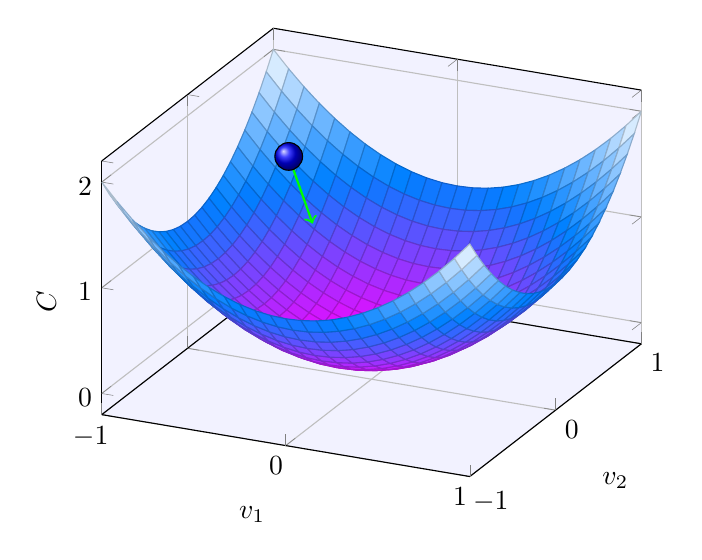
\begin{tikzpicture}
    \begin{axis}[
      %title={$x^2 + y^2$},
      %3d box=complete,
      grid=major,
      axis background/.style={fill=blue!5},
      xlabel=$v_1$,
      ylabel=$v_2$,
      zlabel=$C$,
      xtick distance=1,
      ytick distance=1,
      ztick distance=1,
      xtick={-1,0,1},
      ytick={-1,0,1},
      ztick={0,1,2},
      colormap={cool}{rgb255(0cm)=(255,0,255); rgb255(1cm)=(0,128,255); rgb255(2cm)=(255,255,255)}]

      \addplot3[surf,domain=-1:1] {
        x*x + y*y
      };

      \addplot3[mark=ball,mark size=5pt] coordinates {
        (-0.8, 0.75, 1.2025)
      };

      \draw[->,thick,green] (axis cs:-0.8,0.75,1.2025) -- (axis cs:-0.6, 0.6, 0.72);

    \end{axis}
  \end{tikzpicture} 
\end{document}
